\section*{Bài tập 4.5 --- Naive Bayes}

Giả định \textbf{Naive Bayes}: các thuộc tính trong từng câu \textbf{độc lập có điều kiện} theo lớp. Dùng \textbf{Laplace} với \(\alpha=1\): làm trơn tiên nghiệm và các xác suất điều kiện của thuộc tính \emph{rời rạc}; với từ vựng ở Câu~4.5.4 làm trơn trên \(V=7\) loại từ. Với các biến liên tục (Câu~4.5.1 và~4.5.3), giả thiết phân bố Gaussian trong mỗi lớp với trung bình mẫu và \textbf{độ lệch chuẩn mẫu} (chia \(n_c-1\) khi \(n_c>1\)).

Khi so sánh lớp có thể dùng \(\log\) (tổng log-likelihood + log-prior); hằng số chung không làm thay đổi thứ tự.

%--------------------------------------------------------------------
\subsection*{Câu 4.5.1 --- Phê duyệt tín dụng (biến số + Gia đình)}

Có \(8\) khách hàng huấn luyện, \(|\text{Yes}|=4\), \(|\text{No}|=4\) (theo cột Kết quả).

\subsubsection*{(a) Tiên nghiệm và likelihood}

Hai lớp, làm trơn tiên nghiệm:
\[
P(\text{No})=\frac{4+1}{8+2}=\frac12=0{,}5,\qquad
P(\text{Yes})=\frac{4+1}{10}=\frac12=0{,}5.
\]

Thuộc tính \textbf{Gia đình} (hai giá trị \texttt{Có}, \texttt{Không}): trong lớp \(c\) có \(n_c=4\) khách,
\[
P(\text{giá trị}\mid c)=\frac{\text{số lần xuất hiện trong }c+1}{n_c+2}.
\]
Đếm: lớp \textbf{No} có \(2\) lần \texttt{Có} và \(2\) lần \texttt{Không}, nên
\[
P(\text{Có}\mid\text{No})=\frac{3}{6}=\frac12,\qquad
P(\text{Không}\mid\text{No})=\frac12.
\]
Lớp \textbf{Yes} có \(3\) lần \texttt{Có} và \(1\) lần \texttt{Không}, nên
\[
P(\text{Có}\mid\text{Yes})=\frac{4}{6}=\frac23,\qquad
P(\text{Không}\mid\text{Yes})=\frac13.
\]

Các biến \textbf{Tuổi}, \textbf{Thu nhập}, \textbf{Số tiền vay} coi là liên tục. Ký hiệu lớp chữ thường \texttt{yes}/\texttt{no} cho chi tiết tính toán, nhưng ý nghĩa vẫn là Kết quả \texttt{Yes}/\texttt{No} của đề.

\medskip
\noindent\textbf{Lớp no} (\(4\) mẫu): \\
\(\mu_{\text{age}}=25{,}75\), \(s_{\text{age}}=4{,}5\); \\
\(\mu_{\text{inc}}=19{,}75\), \(s_{\text{inc}}\approx 3{,}594\); \\
\(\mu_{\text{loan}}=235\), \(s_{\text{loan}}\approx 36{,}968\).

\medskip
\noindent\textbf{Lớp yes} (\(4\) mẫu): \\
\(\mu_{\text{age}}=28{,}5\), \(s_{\text{age}}\approx 5{,}066\); \\
\(\mu_{\text{inc}}=19{,}25\), \(s_{\text{inc}}\approx 2{,}217\); \\
\(\mu_{\text{loan}}=145\), \(s_{\text{loan}}\approx 26{,}458\).

\noindent Mật độ Gaussian (mỗi biến):
\[
f(x\mid c)=\frac{1}{\sqrt{2\pi}\,s}\exp\Bigl(-\frac{(x-\mu)^2}{2s^2}\Bigr).
\]

\subsubsection*{Phân lớp mẫu mới}

Mẫu cần dự đoán: Tuổi \(=23\), Gia đình \texttt{Có}, Thu nhập \(=32\) (triệu đồng), Số tiền vay \(=250\) (triệu đồng).

So sánh \(\log P(\text{No})+\log P(\texttt{Có}\mid\text{No})+\sum \log f(\cdot\mid\text{No})\) với tương tự cho \texttt{yes}. Tính đầy đủ từng hạng tử cho ra:
\[
\log \tilde P(\text{No})\approx -16{,}614,\qquad
\log \tilde P(\text{Yes})\approx -34{,}546.
\]
Giá trị \(\log\) lớn hơn rõ rệt thuộc lớp \textbf{No}. Vậy dự đoán Kết quả là \textbf{No} (tức không phê duyệt theo nhãn đề bài).

%--------------------------------------------------------------------
\subsection*{Câu 4.5.2 --- Tennis (toàn rời rạc)}

Có \(14\) mẫu: \(|\text{No}|=5\), \(|\text{Yes}|=9\).

\subsubsection*{(a) Tiên nghiệm và likelihood}

\[
P(\text{No})=\frac{5+1}{14+2}=\frac{3}{8}=0{,}375,\qquad
P(\text{Yes})=\frac{9+1}{16}=\frac{5}{8}=0{,}625.
\]

Với thuộc tính rời rạc có \(V\) giá trị trong tập huấn luyện, trong lớp \(c\) có \(n_c\) mẫu:
\[
P(v\mid c)=\frac{\text{đếm}(v\text{ trong }c)+1}{n_c+V}.
\]

\medskip
\noindent\textbf{Lớp No} (\(n_{\text{No}}=5\)):

\begin{center}
{\small
\begin{tabular}{@{}ll@{}}\toprule
Thuộc tính & \(P(\cdot\mid \text{No})\) sau Laplace \\\midrule
Outlook &
  Sunny \(\frac{3+1}{5+3}=\frac12\); Rainy \(\frac{2+1}{8}=\frac38\); Overcast \(\frac{0+1}{8}=\frac18\). \\
Temp &
  Hot \(\frac{2+1}{5+3}=\frac38\); Mild \(\frac{2+1}{8}=\frac38\); Cool \(\frac{1+1}{8}=\frac14\). \\
Humidity &
  High \(\frac{4+1}{5+2}=\frac57\); Normal \(\frac{1+1}{7}=\frac27\). \\
Windy &
  False \(\frac{2+1}{5+2}=\frac37\); True \(\frac{3+1}{7}=\frac47\). \\
\bottomrule
\end{tabular}
}
\end{center}

\noindent\textbf{Lớp Yes} (\(n_{\text{Yes}}=9\)):

\begin{center}
{\small
\begin{tabular}{@{}ll@{}}\toprule
Thuộc tính & \(P(\cdot\mid \text{Yes})\) sau Laplace \\\midrule
Outlook &
  Sunny \(\frac{2+1}{9+3}=\frac14\); Rainy \(\frac{3+1}{12}=\frac13\); Overcast \(\frac{4+1}{12}=\frac{5}{12}\). \\
Temp &
  Hot \(\frac{2+1}{12}=\frac14\); Mild \(\frac{4+1}{12}=\frac{5}{12}\); Cool \(\frac{3+1}{12}=\frac13\). \\
Humidity &
  High \(\frac{3+1}{9+2}=\frac{4}{11}\); Normal \(\frac{6+1}{11}=\frac{7}{11}\). \\
Windy &
  False \(\frac{6+1}{9+2}=\frac{7}{11}\); True \(\frac{3+1}{11}=\frac{4}{11}\). \\
\bottomrule
\end{tabular}
}
\end{center}

\subsubsection*{(b) Mẫu \texttt{(Sunny, Cool, High, Windy=True)}}

\(\tilde P(c)\propto P(c)\,P(\text{Sunny}\mid c)\,P(\text{Cool}\mid c)\,P(\text{High}\mid c)\,P(\text{True}\mid c)\).

Dùng \(\log\): \(\log\tilde P(\text{No})\approx -3{,}956\), \(\log\tilde P(\text{Yes})\approx -4{,}978\). Vậy \textbf{dự đoán: No}.

\subsubsection*{(c) Outlook không có: \texttt{(?, Cool, High, Windy=True)}}

Không quan sát Outlook nên không nhân thêm bất kỳ \(P(\text{Outlook}\mid c)\) nào; chỉ còn
\(\tilde P(c)\propto P(c)\,P(\text{Cool}\mid c)\,P(\text{High}\mid c)\,P(\text{True}\mid c)\).

\(\log\tilde P(\text{No})\approx -3{,}263\), \(\log\tilde P(\text{Yes})\approx -3{,}592\). Vẫn \textbf{dự đoán: No}.

%--------------------------------------------------------------------
\subsection*{Câu 4.5.3 --- Tennis với nhiệt độ và độ ẩm số}

Outlook và Windy rời rạc (Laplace như Câu~4.5.2). \\
Với Temperature và Humidity: dùng \(\mu\), \(s\) mẫu trong từng lớp; mật độ như Câu~4.5.1.

Từ \(14\) mẫu (nhãn \texttt{yes}/\texttt{no}):

\medskip
\noindent\textbf{Tiên nghiệm:} \(P(\text{no})=\frac{3}{8}\), \(P(\text{yes})=\frac{5}{8}\).

\noindent\textbf{Gaussian:} lớp \textbf{no} (\(5\) mẫu): \(\mu_T=74{,}6\), \(s_T\approx 7{,}893\); \(\mu_H=84\), \(s_H\approx 9{,}618\).

Lớp \textbf{yes} (\(9\) mẫu): \(\mu_T=73\), \(s_T\approx 6{,}164\); \(\mu_H\approx 78{,}222\), \(s_H\approx 9{,}884\).

\noindent\textbf{Likelihood rời rạc} cho \texttt{sunny}/\texttt{rain}/\texttt{overcast} và \texttt{true}/\texttt{false} giống cách đếm Laplace trên bảng đề (ví dụ \(P(\text{sunny}\mid\text{no})=\frac12\), \(P(\text{sunny}\mid\text{yes})=\frac14\), v.v.).

\begin{figure}[htbp]
  \centering
  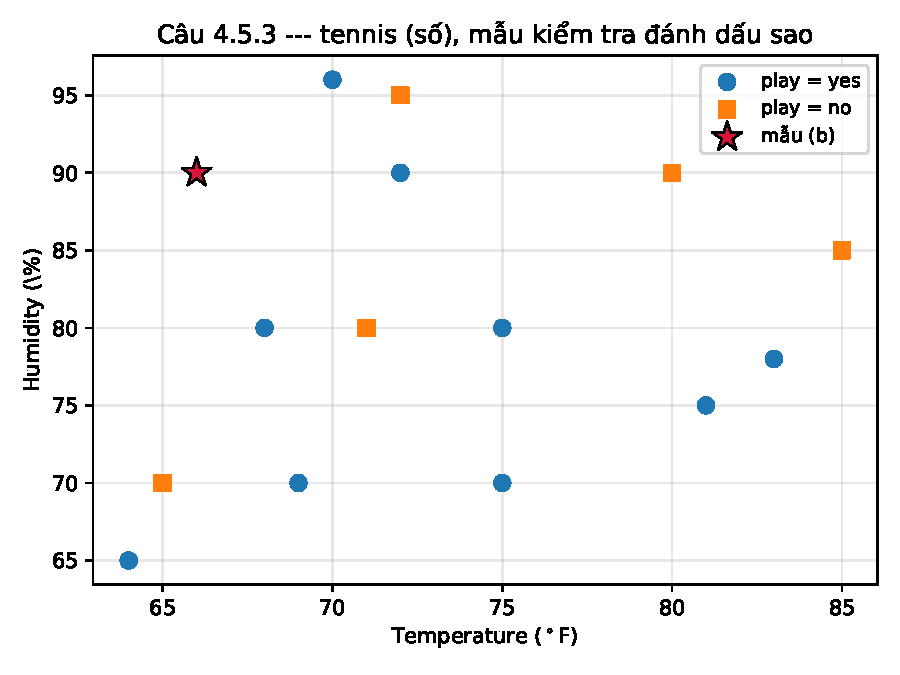
\includegraphics[width=0.72\linewidth]{figures/q_4_5_3_temp_humidity_scatter.pdf}
  \caption{Câu 4.5.3: các điểm huấn luyện theo hai lớp; dấu sao là mẫu cần phân lớp ở phần~(b).}
\end{figure}

\subsubsection*{(b) Mẫu \texttt{(sunny, 66, 90, windy=true)}}

Cộng \(\log\) tiên nghiệm hai mật độ Gaussian (tại \(T=66\), \(H=90\)) và hai xác suất rời rạc. Kết quả:
\[
\log\tilde P(\text{no})\approx -9{,}189,\qquad
\log\tilde P(\text{yes})\approx -10{,}170.
\]
Vậy \textbf{dự đoán: no}.

%--------------------------------------------------------------------
\subsection*{Câu 4.5.4 --- Email: Multinomial Naive Bayes}

Huấn luyện: hai thư \textbf{N}, một thư \textbf{S}; tổng \(3\) văn bản.

\subsubsection*{(a) Tiên nghiệm và likelihood từ}

\[
P(\text{N})=\frac{2+1}{3+2}=\frac{3}{5},\qquad
P(\text{S})=\frac{1+1}{5}=\frac{2}{5}.
\]

Gộp mọi lần xuất hiện từ trong cùng lớp:

\medskip
\noindent\textbf{Lớp N:} tổng token \(=10\) (E1 và E2).
\[
P(w_i\mid \text{N})=\frac{\text{đếm}(w_i)+1}{10+7}=\frac{\text{đếm}+1}{17}.
\]
Cụ thể: \(P(w_1\mid \text{N})=\frac{2}{17}\), \(P(w_2\mid \text{N})=\frac{5}{17}\), \(P(w_3\mid \text{N})=\frac{2}{17}\), \(P(w_4\mid \text{N})=\frac{1}{17}\), \(P(w_5\mid \text{N})=\frac{3}{17}\), \(P(w_6\mid \text{N})=\frac{2}{17}\), \(P(w_7\mid \text{N})=\frac{2}{17}\).

\noindent\textbf{Lớp S:} tổng token \(=5\) (E3).
\[
P(w_i\mid \text{S})=\frac{\text{đếm}+1}{5+7}=\frac{\text{đếm}+1}{12}.
\]
Ví dụ: \(P(w_1\mid \text{S})=\frac{2}{12}\), \(P(w_7\mid \text{S})=\frac{1}{12}\) (và các \(P(w_i\mid\text{S})\) còn lại theo bảng đếm).

\subsubsection*{(b) E4 với bộ đếm \((1,0,0,0,0,0,1)\)}

Chỉ \(w_1\) và \(w_7\) có tần suất dương:
\[
\tilde P(\text{N})\propto \frac{3}{5}\cdot\frac{2}{17}\cdot\frac{2}{17},\qquad
\tilde P(\text{S})\propto \frac{2}{5}\cdot\frac{2}{12}\cdot\frac{1}{12}.
\]
So sánh \(\log\): \(\log\tilde P(\text{N})\approx -4{,}791\), \(\log\tilde P(\text{S})\approx -5{,}193\). Do đó \textbf{dự đoán: N} (không spam).
